{\fontsize{12pt}{22pt} \textbf{Variational Auto-Encoder}\par}

\vspace{5mm}

Variational autoencoders are a combination of three things:

1. Autoencoders

2. Variational Approximation \& Variational Lower Bound

3. "Reparameterization" Trick

\vspace{5mm}

1. Autoencoders

Autoencoders are used to extract features from unlabeled training data. They are new methods for \textbf{dimensionality reduction} and part of neural networks branch.

\vspace{5mm}

\textit{Note}: autoencoders can be used to replace older dimensionality reduction methods such as PCA for several reasons:

- With PCA we usually have to do several plots to display the most important components. Autoencoders can be constructed to reduce the full data down to 2 or 3 dimensions.

- Although, for very large data sets that can’t be stored in memory, PCA will not be able to be performed. The autoencoder construction using keras can easily be batched resolving memory limitations.

- PCA is restricted to linear separation while autoencoders are capable of modelling complex non linear functions.

\begin{center}
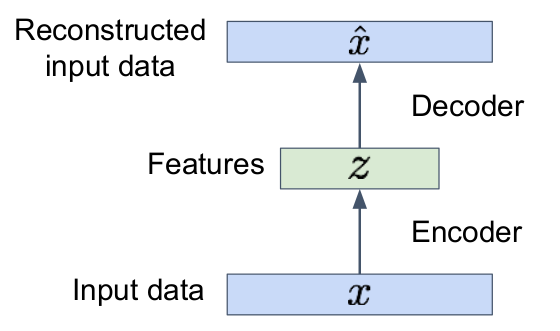
\includegraphics[scale=0.3]{Autoencoders.png}
\end{center}

\vspace{5mm}

Learning can be done using a loss function such as $||x - \widehat{x}||^2$. In a similar way than neural network, optimization is typically done with backpropagation.

\vspace{5mm}

2. Variational Approximation \& Variational Lower Bound

\vspace{5mm}

We assume $x$ is generated from unobserved (latent) $z$:

\begin{center}
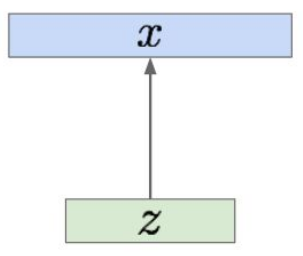
\includegraphics[scale=0.3]{decoder.png}
\end{center}

\vspace{5mm}

\textit{Practical example}: $x$ can be seen as images and $z$ as the main attributes (orientation, colors, etc.)

\vspace{5mm}

$x \sim p_{\theta^*}(x | z)$ where $p_{\theta^*}(x | z)$ is called \textit{true conditional}

$z \sim p_{\theta^*}(z)$ where $p_{\theta^*}(z)$ is called \textit{true prior}

\vspace{5mm}

Objective: estimating $p_{\theta}(x)$. We thus need to estimate $\theta^*$.

\vspace{5mm}

We can do it through maximum likelihood. The marginal density is $p_{\theta}(x) = \int p_{\theta}(x|z) p_{\theta}(z) dz$

\vspace{5mm}

\textit{Note}: a marginal likelihood function is a likelihood function in which some parameter variables have been marginalized. Marginalization consists in summing over the possible values of one variable in order to determine the contribution of another. E.g., $\mathbb{P}(X)=\Sigma_y \mathbb{P}(X, Y=y)$ or in continuous probabilities $p(x)=\int p(x, y) dy$. Also, if we don't know the joint probability, we can express this using conditional probabilities: $p(x)=\int p(x | y) p(y) dy$

\vspace{5mm}

Problem: impossible to compute $p(x|z)$ for every $z$ (\textcolor{orange}{computationally too expensive}) => problem is said \textbf{intractable}

\vspace{5mm}

Solution: use another encoder learning $q_\phi (z|x)$ that approximates $p_\theta(z | x)$

\begin{center}
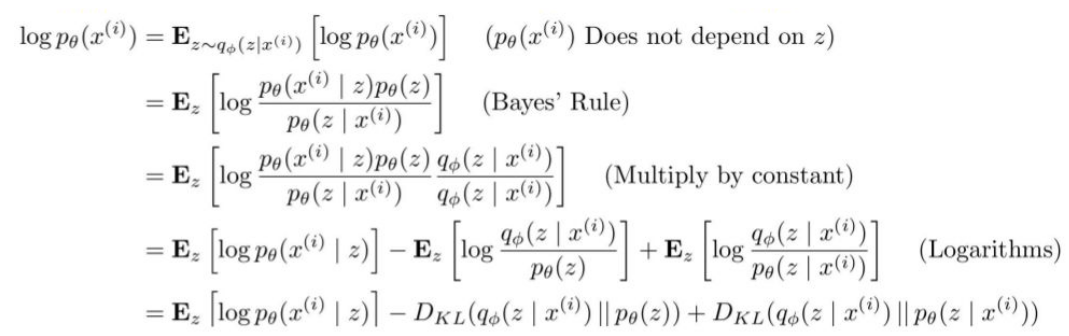
\includegraphics[scale=0.4]{log-likelihood-VAE.png}
\end{center}

\vspace{5mm}

$\mathbb{E}_z[\log p_\theta (x^{(i)} | z]$: we can estimate this term through sampling

$D_{KL}(q_\phi(z | x^{(i)}) || p_\theta(z))$: differentiable term

$D_{KL}(q_\phi(z | x^{(i)}) || p_\theta(z | x^{(i)}))$: $p(z|x)$ intractable but we know that $D_{KL} \geq 0$

\vspace{5mm}

Let $\mathcal{L}(x^{(i)}, \theta, \phi) = \mathbb{E}_z[\log p_\theta (x^{(i)} | z] - D_{KL}(q_\phi(z | x^{(i)}) || p_\theta(z))$ = \textbf{tractable lower bound} that we can optimize

\vspace{5mm}

We know that $p_\theta (x^{(i)}) \geq \mathcal{L}(x^{(i)}, \theta, \phi)$ since $D_{KL}(q_\phi(z | x^{(i)}) || p_\theta(z | x^{(i)})) \geq 0$

Thus the maximum likelihood problem becomes: $\theta^*, \phi^* = argmax_{\theta, \phi} \Sigma_{i=1}^N \mathcal{L}(x^{(i)}, \theta, \phi)$

\vspace{5mm}

We can minimize $D_{KL}(q_\phi(z | x^{(i)}) || p_\theta(z))$ making posterior distribution close to prior. To do so, we make encoder network predicting $\mu_{z | x}$ and $\Sigma_{z | x}$ and then we sample $z | x \sim \mathcal{N}(\mu_{z | x}, \Sigma_{z | x})$

\begin{center}
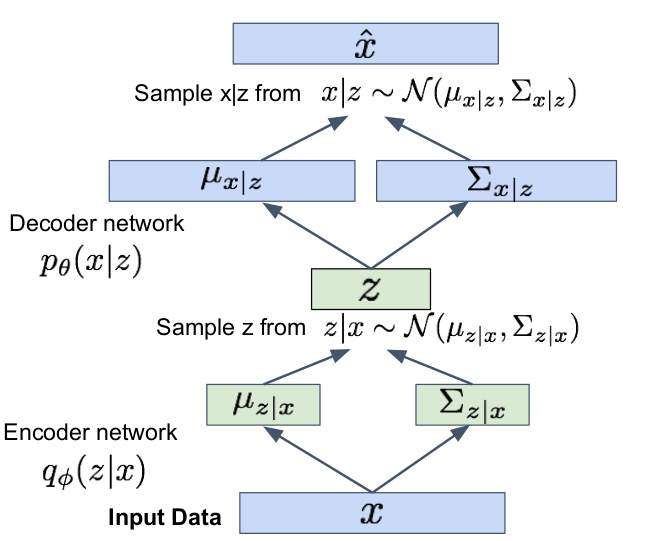
\includegraphics[scale=0.4]{VAE_final_schema.png}
\end{center}

Problem: sampling $z | x \sim \mathcal{N}(\mu_{z | x}, \Sigma_{z | x})$ and $x | z \sim \mathcal{N}(\mu_{x | z}, \Sigma_{x | z})$ is not differentiable (\textcolor{orange}{why?}).

=> we use \textbf{reparametrization trick}: we sample $z_0 \sim \mathcal{N}(0,1)$ to have $z = \mu_{x | z} + z_0 \Sigma_{x | z} \sim \mathcal{N}(\mu_{x | z}, \Sigma_{x | z})$

\begin{center}
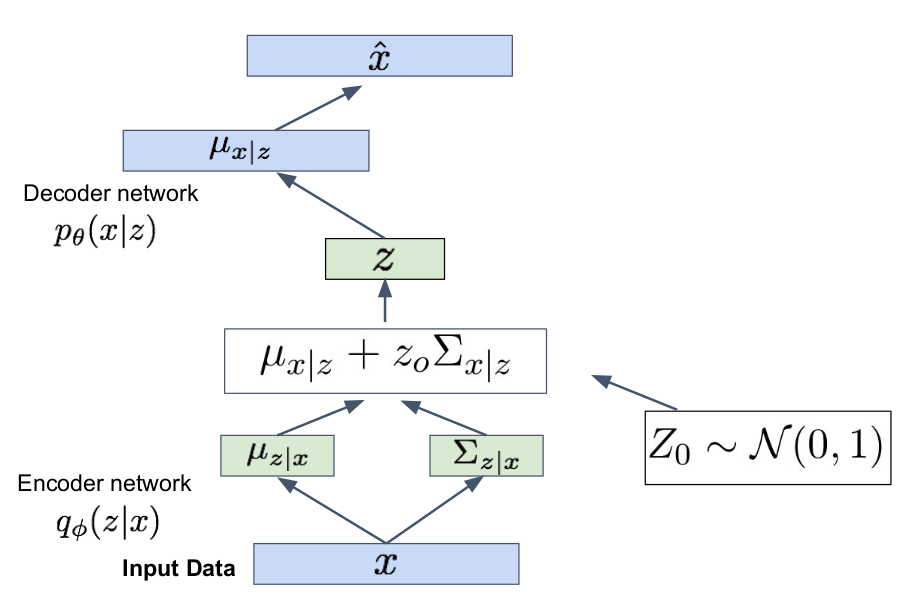
\includegraphics[scale=0.4]{VAE_reparametrization_trick.png}
\end{center}

Optimization through forward and backward propagation!